The rapid advancement of Large Language Models (LLMs) has transformed natural language processing, enabling remarkable text generation and comprehension capabilities. However, open-source LLMs often generate repetitive content, leading to extensive empty lines or recurring sentences, which undermines text quality and fluency. This is particularly problematic in tasks requiring coherent and contextually relevant responses, such as conversational chatbots. To address this, the \textit{repetition penalty parameter} (\rp) is employed during the sampling process to reduce redundant outputs by penalizing previously seen tokens \cite{Keskar2019CTRLAC}. While effective, excessive application of \rp can result in incomplete or fragmented responses, ultimately diminishing user satisfaction.

\begin{figure}
    \centering
    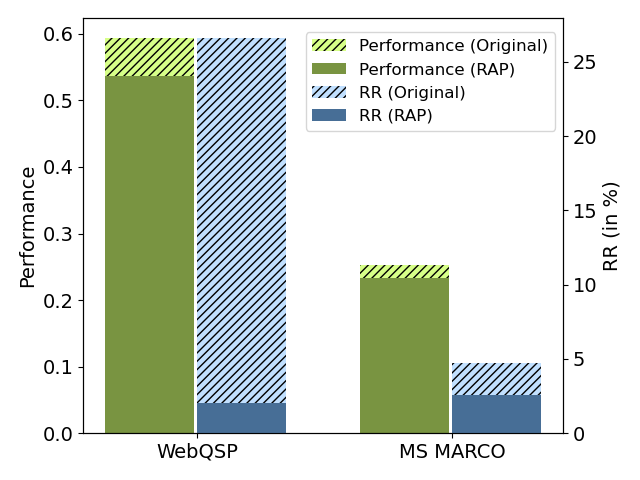
\includegraphics[width=1\linewidth]{image/chart_00_w_legend_Meta-Llama-3-8B-Instruct(RAG - Generic Prompt)_2.png}
    \caption{
    Best performance (F1 for WebQSP, BERT-F1 for MS MARCO) when tuning \rpp using original evaluation metrics (Original) and our proposed repetition-aware performance metric (\rap). \rap helps find \rpp values that minimally reduce performance while significantly lowering repetition ratio (\rr). Result is from Llama-3-8B (RAG-Generic Prompt).}
    \label{fig:hook}
    \vspace{-1.2em}
\end{figure}

% \todo{to rewrite the introduction, remove RF} 
% This paper investigates the intricate interplay between \rp and its impact on generated text. Typically, parameters like \textit{temperature} and \textit{top-k sampling} are optimized through hyperparameter tuning methods such as random or grid search. These methods involve running models with varied parameter values and selecting the best evaluation scores. However, they fail for tuning \rp because traditional metrics like precision, recall, and BLEU scores \cite{papineni2002bleu} overlook repetition. 
This paper explores the relationship between \rpp and its effect on generated text. While parameters like \textit{temperature} and \textit{top-k sampling} are optimized using methods like random or grid search, these fail for tuning \rpp since traditional metrics, such as precision and BLEU scores \cite{papineni2002bleu}, overlook repetition.
% \new{
To address this, we propose a metric called \textbf{R}epetition-\textbf{A}ware \textbf{P}erformance (\rap), which quantifies repetition and penalizes it in the model’s performance evaluation, allowing for the tuning of \rpp. 
Figure \ref{fig:hook} illustrates tuning \rpp for Llama-3-8B using the original evaluation metrics (Original) and our proposed metric. For the WebQSP dataset \cite{yih2016value}, repetition ratio (\rr) is reduced by 93.1\% but the performance only drops by 3.7\%. For the MS MARCO dataset \cite{huang2024performance}, \rr drops by 73.9\% with only 3.7\% of performance drop. Tuning \rpp using \rap can significantly reduce the \rr with minimal performance loss. More examples can be found in Appendix (\ref{sec:how_severe}).

% Figure \ref{fig:hook} shows an example when tuning \rpp for Llama-3-8B using the original evaluation metrics (Original) and our proposed metric (\rap). \rap helps find \rpp values that minimally reduce performance  while significantly lowering repetition ratio. For WebQSP dataset \cite{}, the performance reduces 3.7\%, but the repetition ratio (\rr) reduces 93.1\%. These numbers for MS MARCO dataset \cite{} are 3.7\% and 73.9\%. 
%
% Figure \ref{fig:hook} shows an example of tuning \rpp for Llama-3-8B when using the original evaluation metrics (Original) and our proposed metric. \rap helps in identifying \rpp values that minimize performance reduction while substantially decreasing the repetition ratio (\rr). For the WebQSP dataset \cite{yih2016value}, performance drops by 3.7\%, but the repetition ratio decreases by 93.1\%. For the MS MARCO dataset \cite{huang2024performance}, the performance reduction is 3.7\%, with a 73.9\% decrease in repetition ratio.
%
To compute \rap, we introduce an efficient algorithm called \alg -- Repetition Detection Algorithm--designed to identify all repeating patterns, including non-word character (\nwc) and text repetitions, along with their corresponding repetition lengths. Additionally, we define the repetition ratio (\rr), which measures the proportion of repeated content relative to the total text length. \rr is applied to penalize the model’s performance using a cubic penalty formula, as detailed in Section \ref{sec:method}. Figure \ref{fig:overall} illustrates computing \rap with a running example. 
% Although the accuracy is 100\%, the content has many repeated text that results in reducing the performance to 24.63\%. 
Although the accuracy is 100\%, the content contains many repeated elements, resulting in a low RAP score of 24.63\%.
% }
% quantify repetition by integrating \rf into the model’s evaluation. Using an efficient method based on regular expressions, we measure repetition in LLM responses and compute \rf to penalize performance according to repetition levels. Figure \ref{fig:overall} illustrates \ours with a running example. Although the accuracy is 100\%, the content has many repeated text that results in reducing the \textit{repetition-aware performance} (\rap) to 49.18\%. 
% The repetition factor, combined with a tailored algorithm for detecting repetition patterns, forms a comprehensive framework for optimizing performance while suppressing redundancy. Details are in Section \ref{sec:method}.

% we propose a novel metric called \textit{repetition factor} (\rf), calculated based on the total length of repeated content in the generated text. By incorporating \rf into evaluation metrics, we effectively penalize performance based on the level of repetition in the response.

%
% We propose a framework, namely Repetition-Aware Performance Evaluation for Generated Text (\ours), to quantify repetition by integrating \rf into the model’s evaluation. Using an efficient method based on regular expressions, we measure repetition in LLM responses and compute \rf to penalize performance according to repetition levels. Figure \ref{fig:overall} illustrates \ours with a running example. Although the accuracy is 100\%, the content has many repeated text that results in reducing the \textit{repetition-aware performance} (\rap) to 49.18\%. 
% The repetition factor, combined with a tailored algorithm for detecting repetition patterns, forms a comprehensive framework for optimizing performance while suppressing redundancy. Details are in Section \ref{sec:method}.
%
% We perform a thorough evaluation of nine open-source LLMs with sizes ranging from 2 billion to 70 billion parameters. Our experiments encompass two distinct question-answering (QA) tasks: knowledge base question answering (KBQA) and open-ended question answering (OEQA). For KBQA, we utilize the WebQSP dataset \cite{yih2016value}, where each answer comprises a list of entities from the Freebase knowledge graph. For OEQA, we employ the \ms\footnote{\url{https://microsoft.github.io/msmarco/}} dataset \cite{bajaj2016ms}, which includes real Bing questions and human-generated answers. Given that \webqsp requires entity lists as answers, we introduce an LLM-based evaluation method for KBQA. Specifically, we ask an LLM to extract answer-items (entities) from the generated text and mapping the predicted entities to the ground-truth entities. This approach allows us to use KBQA evaluation metrics, including precision, recall, and F1, as detailed in Section \ref{sec:gemini}. Additionally, we explore the impact of \rp on two prompting strategies: Retrieval-Augmented Generation (RAG)\cite{lewis2020retrieval} and non-RAG. Our study, which covers a diverse range of models, provides valuable insights into the optimal parameter values for balancing performance and repetition suppression in open-source LLMs.
%
\begin{figure*}
    \centering
    % 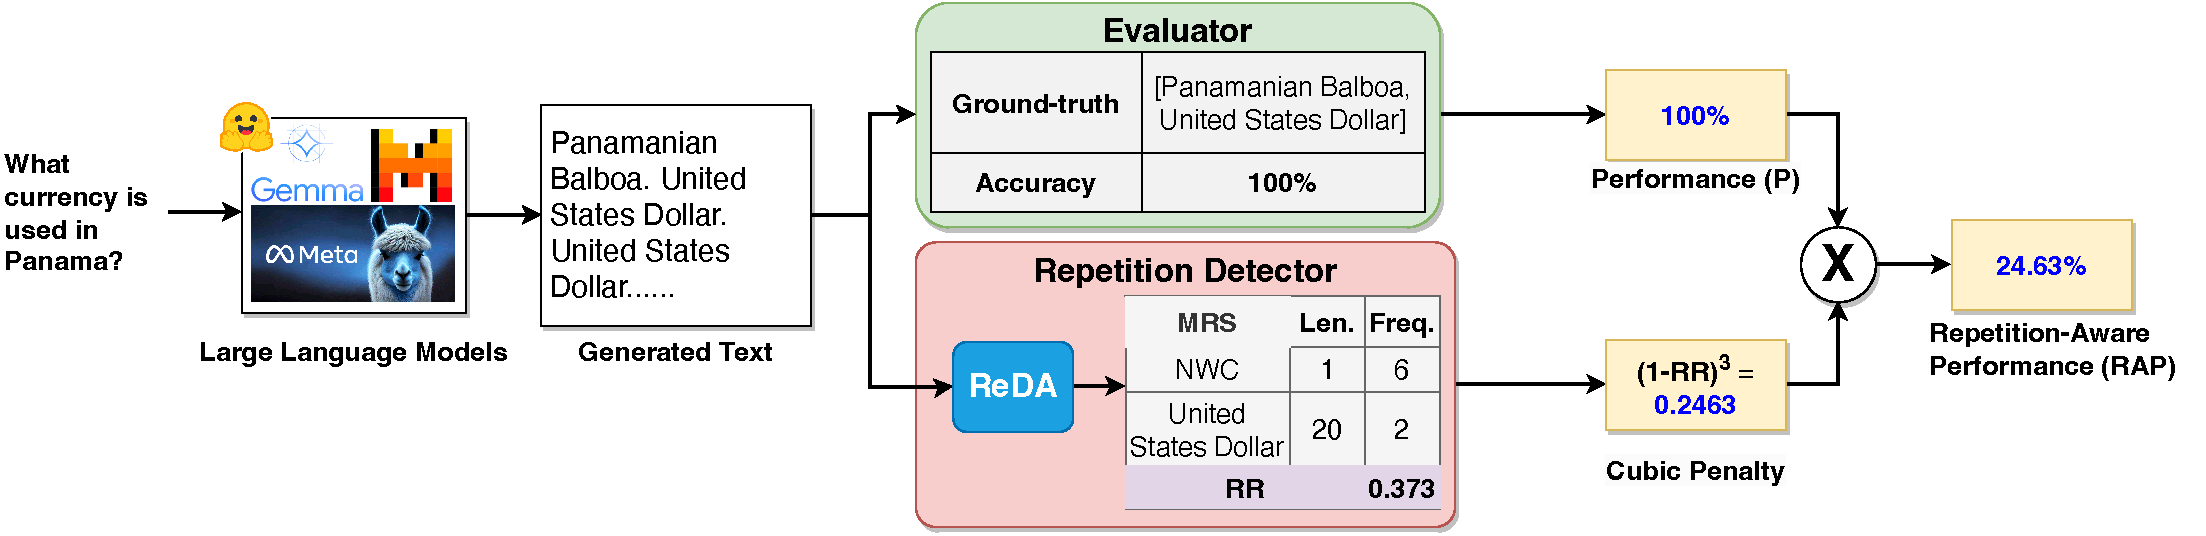
\includegraphics[width=\textwidth]{image/RAPGeT_v4.pdf}
    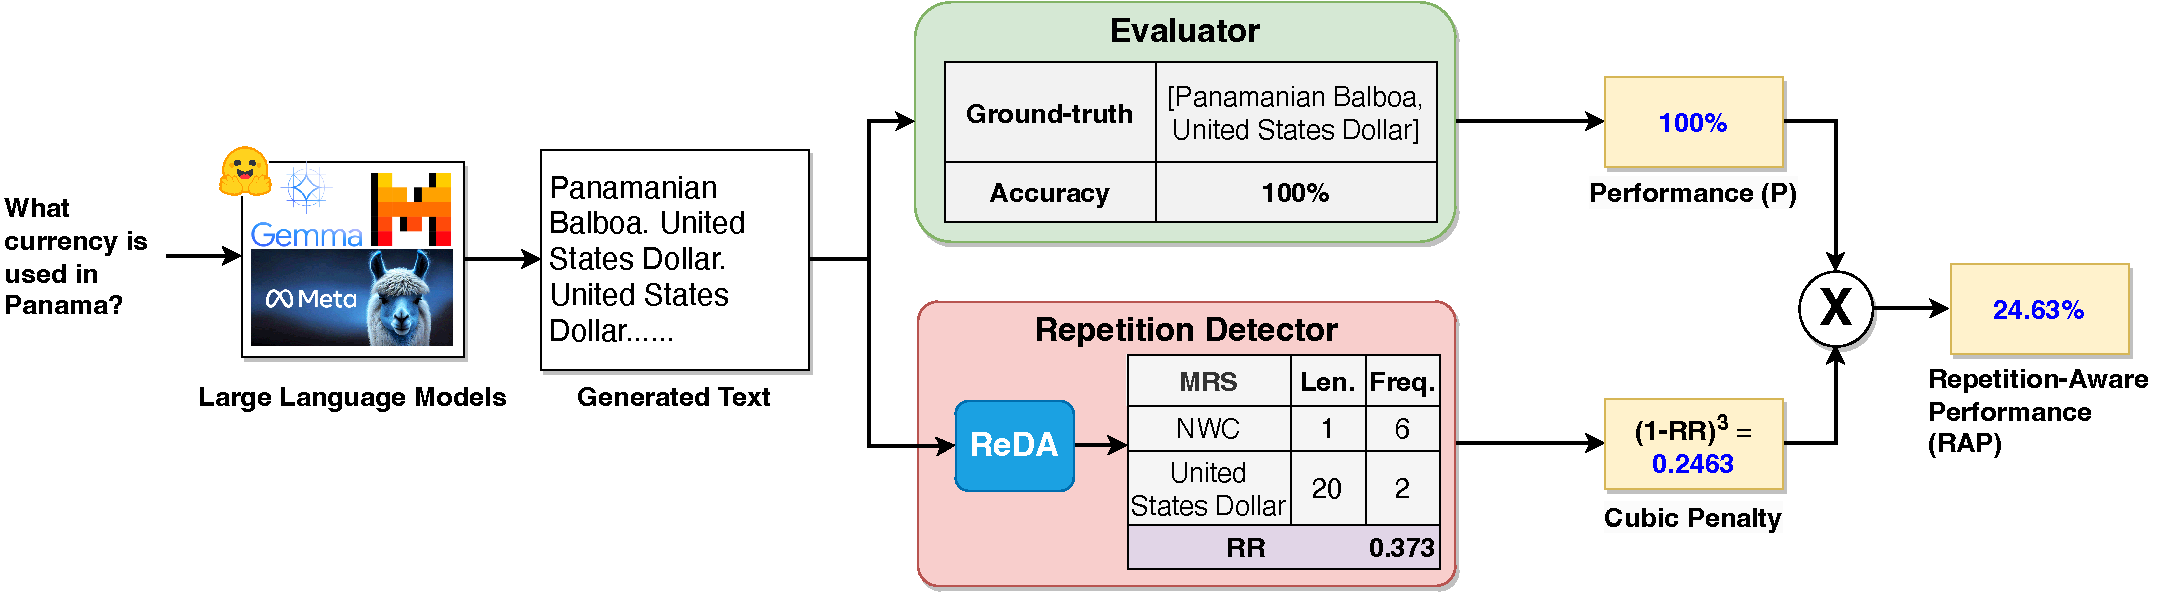
\includegraphics[width=\textwidth]{image/RAPGeT_v3-v5.2.pdf}
    \caption{Overall Methodology: \rap integrates the repetition penalty in the evaluation score. In the example, the generated text contains non-word characters (\nwc) repetition and text repetition. After penalization, the accuracy is reduced from 100\% to 24.63\%. \alg stands for Repetition Detection Algorithm.
    % Repetition-Aware Performance (\rap) integrates a repetition penalty into the evaluation score. In the illustration, the generated text contains non-word character (\nwc) repetition and text repetition, as shown in block (a). Here, \alg stands for the Repetition Detection Algorithm. After applying the repetition penalty, the performance is reduced from 100\% (without detecting repetition) to 24.63\% (after considering repetition). If no repetition is detected in block (a), the RAP score in block (c) will be the same as the performance obtained in block (b), which does not consider the repetition penalty.
    }
        \label{fig:overall}
\end{figure*}

We conduct experiments on three datasets encompassing question answering (including knowledge base question answering--KBQA-- and open-ended QA) and machine translation tasks.
% For question answering, we use \webqsp \cite{yih2016value} (knowledge base QA -- KBQA) and MS MARCO\footnote{\url{https://microsoft.github.io/msmarco/}} \cite{bajaj2016ms} (open-ended QA) datasets. For machine translation, we use \todo{MT-DATASET HERE!}. 
We evaluate twelve open-source LLMs ranging from 2 to 70 billion parameters. 
% For KBQA, answers are lists of entities from the Freebase knowledge graph. 
% As KBQA requires entity lists as answers, we introduce an LLM-based evaluation method for KBQA evaluation. We ask an LLM (\gemini) to extract entities from generated text and map them to ground-truth entities, enabling the use of KBQA metrics like precision, recall, and F1. 
We also examine the effect of repetition suppression for different prompting strategies including Retrieval-Augmented Generation (RAG) \cite{lewis2020retrieval} and non-RAG, combining with generic prompt and chat template.

Our study reveals that increasing \rpp typically reduces repetition but often results in performance degradation, highlighting the importance of tuning \rpp. The effects of \rpp differ across various models, datasets, and prompting techniques. Additionally, we find that using chat templates is effective in reducing repetition for QA task. Our experimental results demonstrate that \rap can effectively tune \rpp, helping to identify a trade-off value that significantly reduces repetition while minimizing performance loss.
These findings offer insights into optimizing \rpp for performance and repetition suppression in open-source LLMs.

This paper presents three key contributions. 
% \begin{itemize}
First, we propose \rap, a novel evaluation metric based on the repetition ratio that quantifies and integrates repetition issues into model performance, enabling the tuning of hyperparameters such as \rpp. We also develop an efficient Repetition Detection Algorithm (ReDA) algorithm for detecting both \nwc and text repetition, addressing  the key challenge in open-source LLMs. 
% Second, we present an LLM-based evaluation method for the KBQA task, which requires entity lists as answers rather than natural language responses. This approach facilitates the evaluation of open-source LLMs without compromising quality by enforcing strict output templates.
Second, we conduct comprehensive experiments on twelve open-source LLMs ranging from 2 to 70 billion parameters, across two tasks--QA and MT--using three datasets and multiple prompting techniques, including RAG and non-RAG methods, with the use of Generic Prompt and Chat Template. These experiments provide valuable insights into reducing repetition while maintaining performance and demonstrate the effectiveness of tuning \rpp using \rap.
Third, we publish all source code and data generated during these experiments at GitHub\footnote{\url{https://github.com/inflaton/rap}}, which includes a significant amount of text produced by open-source LLMs. This dataset is a valuable resource for future research in developing advanced repetition detection methods, assessing LLM capabilities in entity extraction, and evaluating performance in question answering and machine translation tasks.

% Our research provides insights into the trade-offs between repetition reduction and performance degradation when tuning \rpp across different models, datasets, and prompting strategies (such as using generic prompts and chat templates). This can guide future research in optimizing \rpp for open-source LLMs in various use cases.

% \end{itemize}


% \new{Third, we conduct comprehensive experiments on various open-source LLMs on two tasks of QA and MT, using three different datasets, with different prompting techniques of retrieval-augmented generation (RAG) using Generic Prompt and Chat Template, and non-RAG (using Chat Template). 
% The extensive set of experiments provide important insights for reducing repetition without sacrificing too much of performance. The comprehensive set of experiments also demonstrate the effectiveness of tuning \rpp using \rap. 
% Lastly, we will publish all source code and data generated during conducting the experiments shown in this paper. This data contains a substantial amount of text generated by open-source LLMs. It will be a valuable resource for future research, such as developing advanced repetition detection methods, assessing LLM capabilities in entity extraction, and evaluating LLMs performance in QA and ML tasks.


% using two QA datasets with three prompting strategies: RAG with a Generic Prompt, RAG with Chat Template, and non-RAG. Additionally, we use one machine translation (MT) dataset with two prompting strategies: MT with Generic Prompt and MT with Chat Template.} 
% Our findings indicate that higher RPP values generally lead to a reduction of repetition behavior but also impact performance in various ways, necessitating careful tuning of RPP to balance both aspects. 

% This paper makes four key contributions. First, we introduce the repetition factor (\rf) alongside a repetition detection method to directly quantify and incorporate the repetition issue into the model’s performance score, enabling traditional hyperparameter tuning, such as grid search, for the repetition penalty parameter. Second, we present an LLM-based method for evaluating LLM output for the KBQA task, which requires answers in the form of entity lists rather than natural language responses. Third, we conduct comprehensive experiments on a wide range of open-source LLMs using two different QA datasets and two distinct prompting strategies: RAG and non-RAG. Lastly, we will publish all the content generated by the LLMs from our experiments, including their outputs for both the QA tasks and the KBQA evaluation. This dataset, comprising a substantial amount of text generated by open-source LLMs, will be a valuable resource for future research, such as developing more advanced repetition detection methods, assessing LLM capabilities in entity extraction, and evaluating LLM performance in QA tasks.
%%--------------------
% This paper makes four key contributions. First, we introduce the repetition factor (\rf) and a repetition detection method to quantify and incorporate repetition penalty into the model’s performance score, allowing for traditional hyperparameter tuning of the repetition penalty parameter. Second, we present an LLM-based evaluation method for KBQA, which requires entity lists as answers instead of natural language responses. 
% Third, we conduct comprehensive experiments on various open-source LLMs using two QA datasets and three prompting strategies: RAG with Generic Prompt, RAG with Chat Template and non-RAG. 
% \new{Third, we conduct comprehensive experiments on various open-source LLMs using two QA datasets with three prompting strategies: RAG with a Generic Prompt, RAG with Chat Template, and non-RAG. Additionally, we use one MT dataset with two prompting strategies: MT with Generic Prompt and MT with Chat Template.}
% Lastly, we will publish all the content generated by the LLMs from our experiments, including outputs for both QA tasks and the KBQA evaluation. This dataset, containing a substantial amount of text generated by open-source LLMs, will be a valuable resource for future research, such as developing advanced repetition detection methods, assessing LLM capabilities in entity extraction, and evaluating LLM performance in QA tasks.
%---------

% Third, we conduct comprehensive experiments on various open-source LLMs using two QA datasets and three prompting strategies: RAG with Generic Prompt, RAG with Chat Template, and non-RAG. Our findings indicate that higher RPP values generally lead to a reduction of repetition behavior but also impact performance in various ways, necessitating careful tuning of RPP to balance both aspects. Our extensive experiments demonstrate the effectiveness of tuning via our RAPGeT framework. 
% This paper presents four key contributions. First, we introduce RAPGeT, a framework using the repetition factor (RF) and a fast repetition detection algorithm (ReDA) to quantify text repetitions and excessive whitespaces, and incorporate repetition penalties into model performance scores for hyperparameter tuning. Second, we propose an LLM-based evaluation method for KBQA requiring entity lists as answers. Third, our extensive experiments on various open-source LLMs using two QA datasets and three prompting strategies reveal that higher RPP values reduce repetition behavior but impact performance, highlighting the need for careful RPP tuning. Finally, we will publish all source code and datasets for RAPGeT, including LLM-generated content, to support future research in repetition detection, entity extraction, and QA task evaluation.